\chapter{Procedure and Data}

\section{Setup}
\begin{figure}
	\centering
	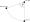
\includegraphics[width=.4\textwidth]{./img/setup.pdf}
	\captiond{The setup}{used in this experiment}
	\label{fig:setup}
\end{figure}
The setup consists of a scintillation detector, consisting of a NaI-scintillator crystal and a sensitive photomultiplier tube (PMT), a small pedestal, the targets are mounted on and the gamma sources themselves.
Sodium iodide is an inorganic scintillator crystal, giving the advantage of most of the gamma rays being observed through the photoelectric effect.

The angle enclosed by the lines of sight detector-target, target-source can be varied to determine the differential cross-section, as seen in \autoref{fig:setup}.

To determine the dependency of the differential cross-section on the atomic number $Z$, four different target materials (Al, Cu, Fe, Pb) are available.

For the dimensions of all materials used in the experiment, see the lab manual (blue book).

\section{Calibration}
\begin{figure}
	\centering
	\includegraphics[width=.5\textwidth]{example-image}
	\caption{Energy calibration}
	\label{fig:calib}
\end{figure}
Every detector channel corresponds to a specific energy.
If an exact linear relationship between channel number and energy is assumed, all that is needed for energy calibration is a gamma source that emits radiation peaks of a known energy.
In this experiment, more than one standard source is used for energy calibration to account for non-linear behavior of the detector.
Using
\begin{equation*}
	E = a\cdot C + b,
\end{equation*}
where $E$ and $C$ denote the channel energy and number respectively, a best fit is applied to determine $a$ and $b$.
Used sources are Co-57, Co-60 and Cs-137.

In \autoref{fig:calib}, known peak energy values are assigned to their corresponding peaks.
Using these values, fit coefficients of
\begin{align*}
	a &= \SI{3.605(22)}{\kilo\eV\per\ch} \\
	b &= \SI{20.23(222)}{\kilo\eV}
\end{align*}
are determined.

\section{Corrections}
For every measurement carried out in this experiment, counts are corrected according to the formula
\begin{equation*}
	N_\text{corr.} = N_\text{obs.} - N_\text{base},
\end{equation*}
where $N_\text{obs.}$ is the observed count and $N_\text{base}$ denotes the baseline noise count for the measurement.

The value for $N_\text{base}$ is acquired by conducting a measurement while the source is isolated by a lead shield.

\section{Errors}
The number of decay events from a radioactive source obeys a Poisson distribution.
For this distribution, a good estimate of its standard deviation is the square root of the count
\begin{equation*}
	\sigma = \sqrt{N_\text{obs.} + N_\text{base}}.
\end{equation*}
This statistic error is assumed for all count rates in this experiment.

\section{Differential Cross-Section}
\begin{figure}
	\centering
	\includegraphics[width=.5\textwidth]{example-image}
	\caption{Differential cross-section over scatter angle}
	\label{fig:diff_cross}
\end{figure}

\autoref{fig:diff_cross} shows the determined differential cross-section $\frac{\d\sigma}{\d\Omega}$ over the scatter angle $\theta$.
For comparison, the theoretical model established in \autoref{eq:kleinnishina} is plotted as well.
It is easy to see that the data is not in accordance with the model.
However, the general shape of the data remotely resembles the model and suggests that an unknown systemic error has not been taken into account.
